


    \section{Gravitational waves in astrophysics}
    \label{grav_waves_astro}

        Space should reverberate with gravitational waves. 
Light shows part of cosmic history; now, primeval epochs and secret stellar reaches might be seen in patterns of light transformed by gravity. 
General Relativity and related theories of gravitation posit~\cite{EinsteinRosen1937} that changing quadropolar masses radiate gravitationally, just as accelerating dipolar charges do electromagnetically. 
In those waves we might see black holes and neutron stars colliding, supernova, the dawn of the Big Bang and rotating neutron stars -- and the potential for unanticipated insights, into other objects or laws of physics, is too tantalazing to ignore. 
As yet, no direct detections are known. 
Hulse and Taylor \cite{HulseTaylor1975} observed a neutron star in a binary system, PSR 1913+16, with an orbit shrinking just as gravitational radiation would entail. 
Following on the pioneering work of Joseph Weber with bar detectors~\cite{Weber1960} and Robert Forward with tabletop interferometers~\cite{Forward1978}, kilometer-scale interferometers were built at the end of the last millenium to look for gravitational radiation. 
Laser light in these instruments travels orthogonal paths and is reflected back; shifts in the combined pattern are scrutinized for indications that gravitational waves stretched space itself. 
This thesis describes efforts to make that search more sensitive with quantum optics at the observatories, by filtering noise from the data, and by conducting a promising search for continuous waves from neutrons stars in binary systems.

Gravitational wave detectors seek to sense vibrations in the metric of spacetime.
Each chapter in this thesis relates to this endeavor.
LIGO, Virgo, and GEO600, soon to be joined by KAGRA, are kilometer-scale intereferometers, gravitational wave antennae standing on the threshold of detection.
Noise intrinsic to the optical configuration of these instruments is subtracted, as exemplified post-facto by LIGO feedforward filtering using recorded servo data in Chapter \ref{chap2}. 
Sensitivity can also be honed by quantum optical squeezing, selecting the relevant uncertainties from Heisenberg's principle, in Chapter \ref{chap3}.
Astrophysicists expect us to find signals from one of four categories of cosmic sources: inspiralling binary systems of stellar remnants, supernovae and similar bursts, stochastic background, and continuous waves from neutron stars.
Einstein's theory predicts the intensity, speed, and polarization of gravitational waves that could be emitted from these sources.
Low-mass X-ray binaries should lead astronomically long lifetimes, radiating continuous waves from their constituent neutron stars, driving our frequentist search of the Fourier-domain.
Chapters \ref{chap4} and \ref{chap5} use these expectations to enhance and run analyses of simulated and real data, particularly for Scorpius X-1 and XTE J1751-305.
Astronomy has grown from humanity's first glimpses into the night sky with the unaided eye. 
With every new instrument, from Galileo's telescope through radio antennae and neutrino detectors, our understanding of the cosmos has grown. 
Communicating that understanding is the subject of Chapter \ref{chap6}.
Gravity pervades the universe like no other force: we must hear its tale. 

        
        \subsection{Cosmic sources of gravitational waves}
        \label{cosmic_sources}
      
        %   --- Cosmic origins believed to generate GW. (note: should sprinkle citations as needed, not just where it says "cite") ---

		Gravity's power to induce ripples in space is a matter of fact. Pulsar 1913+16, discovered by Hulse and Taylor, not only followed a pattern of orbital decay consistent with radiative loss of orbital decay to gravitational radiation -- it continued to do so~\cite{WeisbergTaylor2004,Weisberg2010}, even after Hulse and Taylor won the 1993 Nobel Prize in physics. 
Moreover, there has been much interest in the question of whether the BICEP2~\cite{BICEP2014} and Planck~\cite{Planck2014} probes of the cosmic microwave background have seen evidence of $B$-mode polarizations that would indicate primordial gravitational fluctuations. We still may ask whether the waves are directly detectable on Earth. We may ask whether they appear in detectors in a way consistent with general relativity. The basic fact of their emission, however, appears settled.

	\begin{figure}
	\begin{center}
	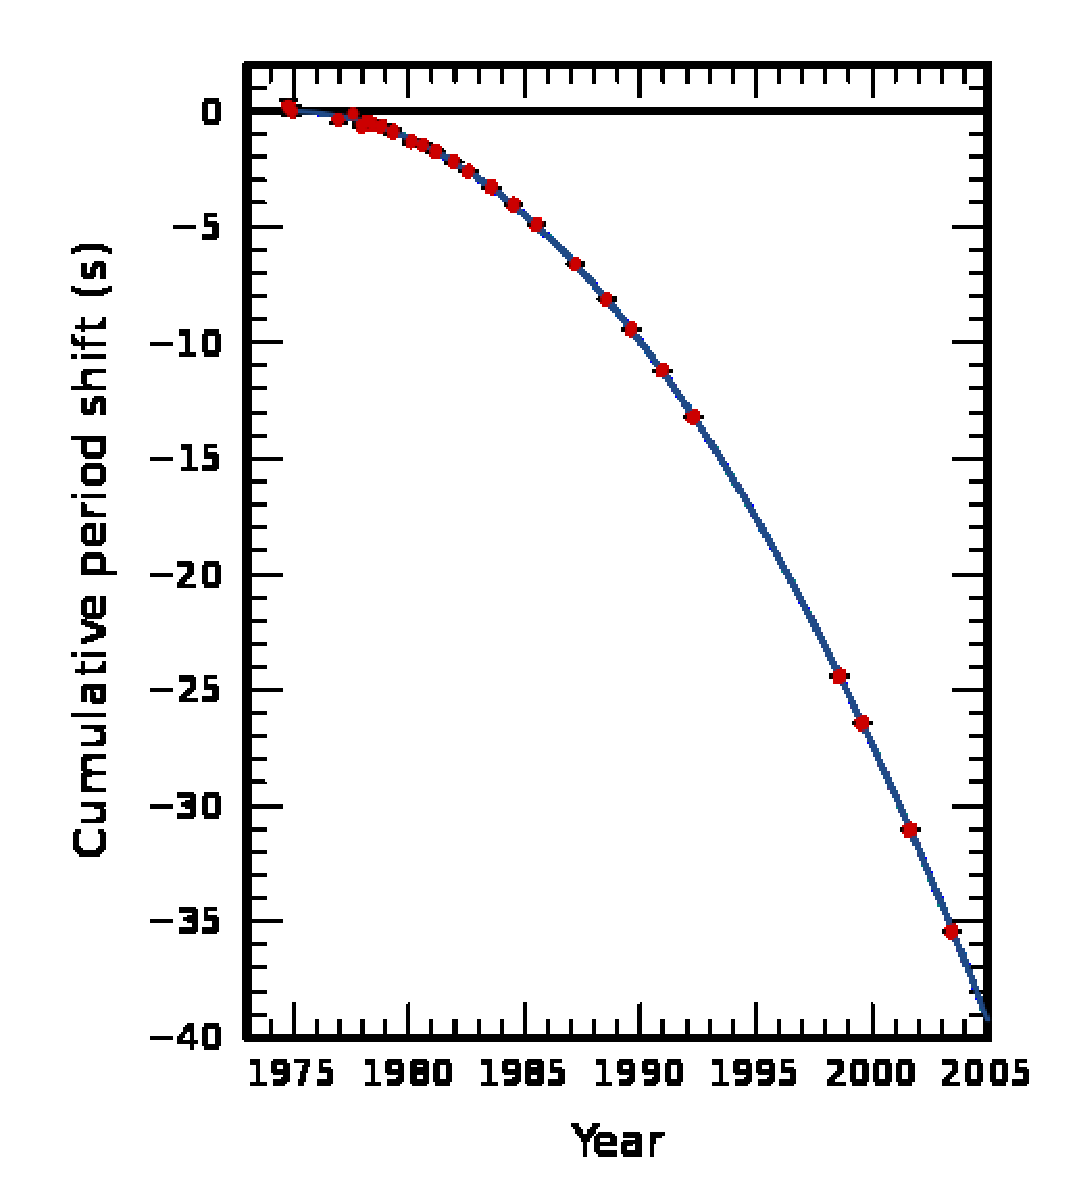
\includegraphics[height=111mm, width=148mm]{500px-PSR_B1913+16_period_shift_graph.eps}
	\caption{The Hulse-Taylor binary, orbital period change over time consistent with emission of gravitational radiation from its system}
	\label{Hulse-Taylor_binary}
	\end{center}
	\end{figure}

		Before delving into the specifics of general relativity, we might consider all the astrophysical sources we expect to emit gravitational waves. Physics prompts our search, but astronomy makes it exciting.

	Discussions of gravitational waves frequently begin with derivations of the wave equations from Einstein's field equations. 
General relativity, however, is not the only theory to predict gravitational waves: waves are a natural consequence of a class of similar theories, which make a range of testable predictions (such as number of polarization modes, from two to six, and possibly speeds different from $c$)~\cite{Will1993} 
Waves should thus be expected even if some minor variation from Einstein's theory is discovered, pointing a way perhaps toward a quantum theory of gravity~\cite{Sathyaprakash2009}. 
As the field progresses toward first detection and beyond to astronomy, the astrophysical targets of our searches should take precedence.

		Gravitational waves (henceforth also abbreviated GW) searches presently focus on four distinct types of cosmic sources.
This categorization of sources was presented in the 1983 LIGO Blue Book proposal and has since guided research focus~\cite{CollinsGravityShadow,Schutz1989}. 

This thesis concentrates on continuous waves, which are sine waves -- perhaps modulated by orbital motion, spin-up or spin-down. 
Continuous waves are most likely to be detectable from neutron stars. 
Given a sufficiently large ellipticity, which might be on the order of $\epsilon \approx 10^{-7}$~\cite{Owen2005} or smaller for a neutron star rotating on the order of 1 kHz, a deformation of the crust would radiate sufficient gravitational radiation to be a plausibly-detectable source. 
Indeed, the radiation would rapidly deplete the rotational energy of the neutron star~\cite{Owen1998}, which is why binary systems, where the neutron star could be recycled and spun-up by a partner, prove a promising target~\cite{PapaloizouPringle1978,Wagoner1984}. 
Scorpius X-1 offers a canonical case~\cite{AbbottScoX12007}, although our discussion of the TwoSpect analysis will elaborate the abundance of other low-mass X-ray binary (LMXB) systems of interest. 
Given the paucity of information on the interiors of collapsed stellar remnants, direct detection of gravitational waves from neutron stars could prove informative. 
Just as we might infer details from neutron star binary coalescences favoring one equation of state~\cite{Lattimer2007,Read2009}, we might also extract parameters from continuous waves suggesting the existence of quark stars or gravitars~\cite{Owen2005}, and will have an unparalleled peek into the interior of the densest stable three-dimensional objects in the universe. 
Their simple waveforms might even facilitate the calibration of other types of gravitational wave data, whereas binary mergers should sound like standard sirens to compare against electromagnetic and neutrino observations~\cite{Punturo2010} 
From any source, continuous waves are a conceptually-elegant and astronomically-enticing target.

		Yet other sources of gravitational waves, as will be discussed in more detail later, have a comparable pull on our attention. Oft discussed, inspirals or compact binary coalescences occur when two stellar remnants draw nearer in their orbits, radiating gravitational radiation and finally merging in a titanic release of energy. While sometimes invisible -- the merging of black holes in short-hard gamma ray burts (GRBs) proving an exception -- these events compete eagerly with supernovae as the most explosive in the modern universe. Were we to detect them directly with gravitational waves, we would see their waveforms, which in turn can be predicted through post-Newtonian approximation and numerical relativity. As the amplitude would diminish linearly with distance, we would then have standard candles or 'sirens' by which to calibrate and measure the universe. Advanced LIGO may prove sensitive to neutron star-neutron star and stellar mass black hole-neutron star mergers, and, if low-frequency sensitivity is sufficient and the sources exist, to intermediate-mass black holes. Space-based observatories such as the longsuffering Laser Interferometer Space Antenna (LISA), the DeciHertz Gravitational-wave Observatory (DECIGO), Big Bang Observer (BBO) and proposed others could detect supermassive black hole mergers. If fortunate, they would see a low-frequency noise floor due not to seismic vibration, as in LIGO, but to white dwarf binaries throughout the galaxy. Since the waveforms are well-predicted, we could even investigate deviations from general relativity, perhaps seeing new physics in the ringdown of black holes.

		Physical insight could also come from burst searches. Bursts share with inspiral searches the property of looking for a single event, as opposed to a source spread over duration. Burst is a somewhat general term, and analyses for them can sometimes be applied to inspiral or detector characterization tasks as well, yet the immediate focus lies with supernovae and perhaps gamma-ray bursts. Because the waveform is unknown, burst searches rely significantly more on the coincidence between multiple detectors to distinguish signal from noise. Just as with neutrino observations of supernova 1987A, the burst program would hope for a fortuitously nearby cataclysm to be seen simultaneously -- or nearly so, the time of flight indicating a direction -- in a global gravitational-wave detector network. Due to the versatility of this method, some researchers have proposed looking for non-general relativitic terms, such as longitudinal polarization in addition to plus and cross orthogonal polarization. Any detection would be quiet exciting for probing systems still mysterious with electromagnetic and neutrino measurements, and it would help, in conjunction with multi-messenger coordinated searches with those observatories, to ascertain at precisely what speed gravity travels through space-time and to what extent it is attenuated or altered.

The background of space-time itself may itself how interesting physics and gravitational wave signatures. Searches for the stochastic gravitational wave background look not for events but for many months of correlated signals between networks of detectors. In doing so, they hope in particular to see the earliest turbulence of the universe -- long before the cosmic electromagnetic background, now microwaves, was emitted 380000 years after the Big Bang, gravitational waves were travelling unimpeded. While the opacity of the infant cosmos conflates electromagnetic signals from different times and places, the transparency of the universe to gravity means that we might see the inflationary epoch or earlier, the Planck time, in gravitational waves. Unfortunately, this signal is thought to be far below the sensitivity of existing detectors. While LIGO did set a new upper limit on the energy density of gravitational waves, measured as a fraction, $\Omega_{gw}$ of the critical closure density of the universe~\cite{LIGOStochasticNature2009}, the inflationary background at LIGO frequencies is predicted to be about ten orders of magnitude lower. Alternative theories, such as ekpyrotic/cyclic universes, make other predictions, so an anomalously high stochastic background could prove cosmologically significant.

All gravitational waves searches look for something. While the most exciting possibility remains that we will see the unexpected, we think that our present divisions will permit serendipity while efficiently categorizing the computational challenges we do expect. Continuous wave and inspiral methods both search against waveform templates; burst and stochastic have no template and rely on correlation and coincidence. Continuous wave and stochastic analyze weeks, months, even years of data in search of persistant features; inspiral and burst look for transient events. In the abstract dimensions of search groups, we are complete. Our blind spots are in what data we provide to those groups -- in the focus on audio frequencies of tens to a few thousand Hertz at present -- blindness that will in time be rectified by CMB polarization, pulsar-timing and space-based interferometry for low frequencies and possibly by atom interferometry for high frequencies. To appreciate our choice of focus in these nascent days of the field, we must turn back a century to understand its origins in Einstein's mathematics.

        \subsection{History from general relativity}
        \label{history_GR}

            %Historical brief of Einstein.
        Einstein's theory unified a sequence of historical insights. Since 1676, when Roemer used the moons of Jupiter to measure the finite speed of light, just before Newton's 1687 \textit{Principia Mathematica}~\cite{Hawking2002}, the question of gravity's propogation beckoned. 
Bringing together the work of Minkowski and Poincar\'{e}, the 1905 special theory of relativity highlighted the naturalness of the speed of light, but only in 1915, with the presentation of the Einstein field equations of general relativity, did a means to an answer emerge. 
In 1916, Einstein predicted gravitational waves. 
At last, gravity had a theoretical speed: the same as that of electromagnetism, that of light in the vacuum, $c$.
In the linear approximation to the nonlinear theory of general relativity (henceforth GR), the waves were mathematically similar to the waves of electromagnetism, as will be shown in Section~\ref{general_relativity}.
Yet the detectability of the waves, even in principle, would remain an open question for another half century. 
Consult Misner, Thorne, and Wheeler's \textit{Gravitation}~\cite{MisnerThorneWheeler} and Sean Carroll's lectures notes~\cite{Carroll1997}, as well as other history books of the field for an account of the controversy.
Riles review~\cite{Riles2013}.
\textit{Gravity's Shadow}~\cite{CollinsGravityShadow} for historical controversy,
\textit{Gravity's Ghost}~\cite{CollinsGravityGhost} for why we do blind injections

Before deriving the answer to the detectability question, a contrast with the situation in other fields of astronomy is in order.

 
        \subsection{Contrast with electromagnetic and particle astronomy}
        \label{contrast_astro}

        With astronomy, detection came first, then theory.

            Contrast with electromagnetism, compare with radio/X-ray/et cetera astro. Can make analogy to radio waves and make note of the ease with which one can operate a small radio telescope, as I did in my thesis~\cite{MeadorsThesis2008}, compared the the difficulty of gravitational wave detection. Muons from space were detected long ago, as in C.D. Anderson's 1949 paper on what was then called the mesotron,~\cite{CDAnderson}. Compare with neutrinos as in the John Bahcall review paper~\cite{NeutrinoReview}, which were a well-established field by the turn of the millenium, including the detection of supernova 1987A. Might be worth comparing to the focus in new neutrino detectors that I had in my research and development work on them~\cite{EBubble2005},~\cite{MeadorsNevis2006}. Even with those detectors, however, astrophysically-oriented detectors could be cross-referenced against terrestrial generators. Bahcall's search for solar neutrinos, which were theoretical in 1964,~\cite{NeutrinosSolarTheoretical}, at least had the certainty that neutrinos had been detected from the Savannah River nuclear reactor. Yet when those solar neutrinos were detected, it a significant confirmation of nuclear theory. General relativity has been established by the 1913+16 pulsar~\cite{WeisbergTaylor2004} and would likely be much boosted by direct detection, and it might reach surprising new insights, analogous to neutrino oscillation found by looking at the solar neutrino spectrum.

    %End section by very rapidly deriving wave equation of electricity and magnetism, to lead by example for how we go about GR.
    %Note that all physics in min(action),
    %introduce metric as inner product
    %generally, coordinate transform good

\subsection{Fields and curvature}
\label{field_curvature_math}

    
    Gravitation as described by general relativity is complex, so let us start with a simpler theory: electromagnetism. 
The same mathematics that predicts electromagnetic waves (light), which are our means of detecting gravitational waves in LIGO, can then be extended by analogy to gravitational waves.
This derivation is detailed so that the gravitational analogue can be expressed more simply.
Definitions follow Carroll~\cite{Carroll1997}

    Let us set geometric, natural units where $1/4\pi\epsilon \rightarrow 1$, $c \rightarrow 1$, $G \rightarrow 1$. 
Greek indices indicate four dimensions, Latin indices three, unless specified otherwise.
Assume the Einstein summation convention, e.g., $x_i y^i \equiv \Sigma_{i=0}^3 x_i y^i$
Anti-symmetrization of indices can be indicated by subscripted square brackets (n.b., all differential forms are antisymmetric), symmetrization by parentheses.

Vectors are typical expressed by reference to index, e.g., a vector $v^\mu$, although implicitly a geometrical vector includes its basis vectors, $e^\mu$ such that $\textbf{v} = v^\mu e_\mu$.
Note that when the vector indices are contravariant, the basis vectors are covariant.
Let subscript commas indicate ordinary partial derivatives, i.e., $x_{,i}^j \equiv \partial_i x^j$.
Semicolons will indicate covariant derivatives (explained in Section~\ref{general_relativity}), which reduce to commas (partial derivatives) in flat space. 
Suppose we work in a space supplied with a metric tensor, $g_{\mu\nu}$, which acts as a bilinear operator (generalizing the inner product) to produce infinitesimal arclength $ds$ according to $ds^2 = g_{\mu \nu} dx^\mu dx^\nu$ for infinitesimal lengths $dx^\mu$ in the direction of, and dual to, basis vectors $e_\mu$. 
The metric allows index raising and lowering, e.g., $g_{\mu \nu} x^\mu = x_\nu$, $g^{\mu \nu} x_\mu = x^\nu$.

Vectors and matrices cann be indicated by boldface, e.g., $\textbf{v} = v^\mu e_\mu$ is a vector, $\textbf{M} = M^{\mu\nu} e_\mu e_\mu $ is a matrix, whereas differential forms (dual to vectors) can be indicated by sans serif, e.g., $\textsf{v} = v_\mu dx^\mu$ is a 1-form, $\textsf{M} = M_{\mu\nu} dx^\mu \wedge dx^\nu$ is a differential 2-form.
Tensors generalize vectors and differential forms, including both co- and contra-variant components, and can be built from tensor products $\otimes$, such as $T^{\mu\nu}_{\rho\sigma} = (\textbf{M})\otimes (\textsf{N}) = (M^{\mu\nu}) \otimes (N_{\rho\sigma})= (\textbf{u}^\mu \otimes \textbf{v}^\nu) \otimes (\textsf{x}_\rho \otimes \textsf{y}_\sigma)$.

The wedge $\wedge$ is the exterior or Grassman product, the antisymmetric operator on differential forms that generalizes the cross product, e.g., for the wedge of two 1-forms, $\textsf{v} \wedge \textbf{w} = -\textsf{w} \wedge \textsf{v}$.
Generally, for $p$-form $\textsf{A}$, $q$-form $\textsf{B}$, $(A \wedge B)_{\mu_1 \cdots \mu_{p+q}} = (p+q)!/(p!q!) A_{[\mu_1\cdots\mu_p} B_{\mu_{p+1} \cdots \mu_{p+q} ]}$. 
The Levi-Civita symbol is $\epsilon_{\mu_1 \cdots \mu_n}$, in $\mathbb{R}^n$, $+n$ for even permutation, $-1$ for odd, $0$ otherwise.
The Hodge star maps differential $k$-forms in an $n$-dimensional space to $n-k$-forms, e.g., in 3-space, $\star dx = dy \wedge dz$, $\star dy = dz \wedge dx$, $\star dz = dx \wedge dy$, or from a scalar $f$, $\star f = (f) dx \wedge dy \wedge dz$, generally in $n$-space, $(\star \textsf{A})_{\mu_1 \cdots \mu_{n-p}} = 1/(p!) e^{\nu_1 \cdots \nu_p}_{\mu \cdots \mu_{n-p}} \textsf{A}_{\nu_1 \cdots \nu_p}$.

Index raising and lowering creates a homology between vectors and differential one-forms, $e_\mu \leftrightarrow dx^\mu$ (for coordinate-free math, this is implicit).
By itself, $d$ indicates the exterior derivative; $df$ of a scalar (0-form) $f$ is (modulo homology) its gradient $\nabla$, and $d\textsf{a}$ maps a $k$-form to a $(k+1)$-form, but $d^2$ is always 0.
Precisely, $(d\textsf{A})_{\mu_1 \cdots \mu_{p+1}} = (p+1) \partial_{[\mu_1} \textsf{A}_{\mu_2 \cdots \mu_{p+1}]}$. 


The divergence $\nabla \cdot$ of a vector field $\textbf{X}$ is homologously given by $\star d \star \textbf{X}$, the curl $\nabla \times$ by $\star d \textbf{X}$, and the Laplacian $\nabla^2$ (in 3-space) or d'Alembertian $\Box$ (in 4-space) of a scalar function are given by $\star d \star f$.
Covariant exterior derivatives will be noted by $D \textsf{v} = d \textsf{v} + \omega \wedge \alpha$ for a differential form $\textsf{v}$ and a \textit{connection} $\omega$ (Section~\ref{general_relativity}); this derivative reduces to $d\textsf{v}$ in flat space.

The usual, coordinate basis vectors set $e_\mu = \partial_\mu$.

Modern physical theories are usually described as extremizing an action, $\mathcal{S}$. 
The action is defined as the integral, over space-time, of a Lagrangian density $\mathcal{L}$. 
To integrate, the integral generally requires a metric, $g_{\mu\nu}$.
Writing the determinant of the metric as $|g| = \det(g_{\mu\nu})$, the action to be extremized (setting $\delta \mathcal{S}$ to 0) is

\begin{equation}
\mathcal{S} = \int \mathcal{L} \sqrt{-|g|} d^4 x.
\end{equation} 

The minus sign accounts for the $-1$ in the Minkowski metric, which physically corresponds to the hyperbolic transformation between space and time in special relativity.
Whereas the usual $\mathbb{R}^3$ Euclidean metric below is $g_{ij}$, the Minkowski $\mathbb{R}^{1,3}$ metric is $\eta_{\mu\nu}$:

\begin{eqnarray}
g_{ij} = \mathbb{I}^3 = 
\left[
\begin{array}{ccc}
1 & 0 & 0 \\
0 & 1 & 0 \\
0 & 0 & 1
\end{array} \right],
\textup{ }
\eta_{\mu\nu} =
\left[
\begin{array}{cccc}
-1 & 0 & 0 & 0\\
0 & 1 & 0 & 0 \\
0 & 0 & 1 & 0\\
0 & 0 & 0 & 1
\end{array} \right].
\end{eqnarray}

Given a Minkowski metric $\eta_{\mu' \nu'}$, a curved 4-space $\mathbb{R}^{1,3}$ metric can be written in \textit{vielbein} terms: $e^{\mu'}_{\mu}$, $e^{\nu'}_{\nu}$ such that $g_{\mu\nu} = e^{\mu'}_{\mu} e^{\nu'}_{\nu} \eta_{\mu' \nu'}$.


The question then becomes how we can define the Lagrangian density for different physical theories. 
In both electromagnetism and gravitation, the quantity is a kind of curvature, contracted from respectively the Maxwell and Ricci tensors. 
This curvature, analogous to an energy term, is then extremized subject to a conserved source term: 4-current in electromagnetism, stress-energy and the cosmological constant in general relativity.

As educated coordinate transformations make a great number of problems simpler -- a theme of the both the feedforward regression and the data analysis presented in later chapters of this thesis -- let us proceed with the derivation in a way that is manifestly covariant under transformations. If desired, one can then extend this treatment to electromagnetism in curved spacetime, such as under the influence of a gravitational wave. 

    Electromagnetism is theoretically defined by a 1-form $\textsf{A} = A_\mu d x^\mu$ where $A^\mu$ is a vector potential~\cite{MisnerThorneWheeler} given by $A_\mu = (\phi, -A_x, -A_y, -A_z)$~\cite{GriffithsE}. 
The scalar electric potential is $\phi$ and the magnetic vector potential is $A_i$.
In a given gauge $\phi$, the theory is \textit{gauge symmetric} ($\phi$ invariant) such that the addition of the differential $d \phi$ to $\textsf{A}$ does not change the theory. 
This changeless symmetry, in the group $U(1)$, arises because the physics of the theory can be described through the derived Maxwell field tensor $F_{\mu \nu}$, or curvature form $\textsf{F}$:

\begin{eqnarray}
\textsf{F} = d \textsf{A} = (\partial_\mu A_\nu) dx^\mu \wedge dx^\nu = \frac{1}{2} F_{\mu\nu} dx^\mu \wedge dx^\nu, \\
F_{\mu \nu} = A_{\nu,\mu} - A_{\mu,\nu},
\end{eqnarray}

By the usual flat-space definitions of potential for an electric field $E$ and magnetic field $B$, $E_i = -\phi_{,i} - A_{i,0}$, $B_i = \epsilon_{ijk} \partial^j A^k = \epsilon_{ijk} A^{k, j}$. 
Electrodynamics in curved space are well-studied; many equations can be translated by replacing partial with covariant derivatives.
Therefore, the Maxwell tensor in explicit coordinate form is

\begin{equation}
F_{\mu\nu} =
\left[
\begin{array}{cccc}
0 & E_x & E_y & E_z\\
-E_x & 0 & -B_z & B_y \\
-E_y & B_z & 0 & -B_x\\
-E_z & -B_y & B_x & 0
\end{array} \right].
\end{equation}

\noindent Maxwell's theory then corresponds to the minimization of the action, finding $\delta S = 0$,


\noindent for a Lagrangian $\mathcal{L}$ with a stress-energy term for the field itself constrained by an interaction with the current 1-form $\textsf{J} = J_\mu d x^\mu$:

\begin{eqnarray}
%\mathcal{L} = - \frac{1}{4} F^{\mu \nu} F_{\mu \nu} + J_\mu A^\mu,\\ 
\mathcal{S} = \int \left( -\frac{1}{4} F^{\mu \nu} F_{\mu \nu} + J_\mu A^\mu \right) \sqrt{-|g|}d^4 x.
\end{eqnarray}

A Hodge dual $\star$ then defines the dual to the Maxwell form, $\textsf{G} \equiv \star \textsf{F}$. 
Maxwellian electromagnetism then is concisely described by extremizing the action to derive the following equations:

\begin{eqnarray}
d \textsf{F} = 0,\\
d \star \textsf{F} = 4 \pi \star \textsf{J}.
\end{eqnarray}  

Applied in flat space, where $g_{\mu \nu} = \eta_{\mu \nu}$, and substituting in the explicit coordinate form of the Maxwell tensor, the theory is easily expressed as four familiar first-order differential equations of the $\textbf{E}$ and $\textbf{B}$ fields in terms of electrical charge density $\rho$ and 3-current $J^i$ (cf. the textbook by Jackson~\cite{JacksonEM}), in (1 time)+(3 space)-dimensions:
 
%(CHECK SIGNS AND UNITS AND FONTS)

\begin{eqnarray}
\star d \star \textbf{E} = E^i_{,i} = \rho,\\
\star d \textbf{E} + \partial_t \textbf{B} = \epsilon^{ijk} E^{k,j} + B^i_{,0} = 0,\\
\star d \star \textbf{B} = B^i_{,i} = 0,\\
\star d \textbf{B} - \partial_t \textbf{E} = \epsilon^{ijk} B^{k,j} - E^i_{,0} = 4 \pi J^i.
\end{eqnarray}

Returning to four full dimensions and specifying the \textit{Lorenz gauge}, where we choose any vector potential for which $\star d \star \textsf{A} = A^\nu_{,\nu} \equiv 0$, 

\begin{eqnarray}
\star d \star d \textsf{A} = -4\pi \textsf{J},
%g^{\mu\nu}A^\sigma_{,\mu\nu} = -4\pi J^\sigma,
\end{eqnarray}
        
\noindent with $\Box \equiv \partial_\mu \partial^\mu$, this is often written as $\Box A^\sigma = -4 \pi J^\sigma$ -- a wave equation. 
This derivation has been laborious in order to establish how differential forms allow a cleaner expression of electromagnetism; the differential form equation also is covariant, accurate in curved spacetime.
Our task now is to compare with general relativity to see whether a similar wave equation will emerge.

    \section{General relativity}
    \label{general_relativity}

        Einstein's theory of General Relativity (hence GR) describes gravitation as a pseudoforce. 
Unlike Newton, Einstein posits that objects always follow an extremized path -- a geodesic worldline -- if the curvature of spacetime is considered. 
This supposition follows from the Fermat principle of least time (in turn, the inspiration for the least action principle, $\delta S = 0$).
Likewise, the following discussion of gravitational wave interferomter is best understood in terms of phase or \textit{time-of-flight}.
The curvature of spacetime is described by the Riemann tensor, $R^\mu_{\nu\rho\sigma}$, which is a solution to the Einstein field equations. 
In Section~\ref{field_equations} the connection between these field equations and the Ricci scalar curvature will be clarified. 
This Riemann tensor can be constructed from the Christoffel connection, $\Gamma^\mu_{\rho\sigma}$, which in turn can be expressed in terms of the metric, $g_{\mu \nu}$.
Whereas electromagnetism arises from $U(1)$ unitary Lie group gauge symmetries, general relativity arises from $GL(4, \mathbb{R})$ general linear Lie group symmetries.

 Carroll and \textit{Gravitation} are essential references~\cite{Carroll1997,MisnerThorneWheeler}, consulting other sources for the Einstein-Hilbert/Palatini action~\cite{FarrThesis}.

%            Introduce the metric $g$ here, but reinforce that it is not essential.
%Intro to GR -- right motivation is least action Ricci tensor, implying field equation and phase/time-of-flight implying interferometry.

        \subsection{Symmetry and action principles}
        \label{principles}

            Like electricity and magnetism, GR is the product of symmetry, action. 


        \subsection{Derivation of field equations}
        \label{field_equations}

            A common approach to gravitational wave derivations is linearized GR~\cite{FlanaganHughes2005}.
            This approach is correct in weak fields, and proceeds~\cite{AdhikariThesis} from the metric $g$ approximation as the sum of a Minkowski (flat spacetime) component, $\eta$, plus a perturbation $h$, where $|h| \ll |\eta|$:

\begin{equation}
g_{\mu \nu} \approx \eta_{\mu \nu} + h_{\mu \nu},
\end{equation}

\noindent leading to a wave equation,

\begin{equation}
-\frac{1}{2} \Box \left(h_{\mu \nu} - \frac{1}{2} \eta_{\mu \nu} h_{\lambda}^{\lambda} \right) = \frac{8 \pi G}{c^4} T_{\mu \nu}.
\end{equation}

The wave carries energy~\cite{BallmerThesis} as well:

\begin{eqnarray}
\rho_{\textup{gw}} = \frac{c^2}{16 \pi G} \left\langle |\partial_t h_+|^2 + |\partial_t h_\times|^2 \right\rangle,\\
P = \frac{G}{5c^5}\left\langle \left( \partial_t^3 I_{ij}\right)^2  \right\rangle \approx 5.5\times 10^{-54} W^{-1} \left\langle \left( \partial_t^3 I_{ij}\right)^2  \right\rangle.
\end{eqnarray}

Let us demonstrate this result and also derive field equations from the action, integrating over extremized curvature~\cite{FarrThesis}.
Obtain the action from Ricci scalar curvature $R$, a hypothetical constant, $\Lambda$ (termed the cosmological constant), and the matter Lagrangian density $\mathcal{L}_M$:

\begin{equation}
\delta \mathcal{S} = \delta \int \left( R - 2\Lambda + \mathcal{L}_M \right) \sqrt{-|g|}d^4 x,
\end{equation}

Given $R = R^\mu_\mu$ Ricci scalar a for a $R_{\mu\nu} = R^\lambda_{\mu\lambda\nu}$ Ricci tensor contracted from the Riemann tensor, $R^\mu_{\nu\rho\sigma}$ (the curvature tensor, equivalently the 2-form $\textsf{R}^\mu_\nu$), we can construct the Maurer-Cartan structure equation with a connection $\omega$,

\begin{eqnarray}
\textsf{R}^\mu_\nu = d\omega^\mu_\nu + \omega^\mu_\rho \wedge \omega^\rho_\nu, \\
\omega^{\rho'}_{\mu\sigma'} = e^{\alpha'}_{\nu} e^{\lambda}_{\beta'} \Gamma^{\nu}_{\mu\lambda} - e^{\lambda}_{\beta'} \partial_{\mu} e^{\alpha'}_{\lambda},\\
\Gamma^\sigma_{\mu\nu} = \frac{1}{2} g^{\sigma\rho} \left( \partial_\mu g_{\nu \rho} + \partial_\nu g_{\rho \mu} - \partial_\rho g_{\mu\nu} \right). 
\end{eqnarray}

\noindent where the last equation defines the \textit{Christoffel} connection. Then we obtain the \textit{Einstein field equations}, sourced by the stress-energy tensor, $T_{\mu\nu}$:

\begin{equation}
R_{\mu} - \frac{1}{2} R g_{\mu\nu} + \Lambda g_{\mu\nu} = 8 \pi T_{\mu\nu}.
\end{equation}

\noindent These are nonlinear, but when linearized, there is indeed a wave solution: $\Box h_{\mu\nu} = 0$~\cite{Carroll1997}
The wave, parametrized by path $x^\mu (\lambda)$ follows the usual geodesic equation, where the covariant derivative by $\mu$ of $V^\nu$ is defined by $\nabla_\mu V^\nu = (\partial_\mu V^\nu + \Gamma^\nu_{\mu\lambda} V^\nu)$ and along a path by $D_\lambda = dx^\mu_\lambda \nabla_\mu$,

\begin{equation}
D_\lambda \partial_\lambda x^\mu = 0
\end{equation}



        \subsection{Radiation from quadrupoles}
        \label{radiation}
  
            Predict power from rotating quadrupole. Might also be a good place to invoke Vladimir's thesis~\cite{DergachevThesis} as well as original primary sources. Note that just as light travels at the speed of light, which is measureable~\cite{CODATA} and which can be derived from electromagnetic theory~\cite{GriffithsE}, so we think that gravity should travel at the speed of light. Note that this radiation should not be affected by the interstellar medium. I think that Ostriker is the source to reference on the ISM~\cite{Caldwell1981},~\cite{McKee1977}.

    \section{Astrophysical estimates}
    \label{estimates}

        Astrophysical estimates and predictions.

        \subsection{Sources: burst, continuous, inspiral and stochastic}
        \label{source_types}

            %Describe the four types of sources: burst, continuous, inspiral and stochastic.

            Let us summarize, more briefly, the current state of the art in each search, describing the four types of searches: burst, continuous, inspiral, and stochastic, with reference to a review by Riles~\cite{Riles2013}.

		Mostly above, but clarify exact how much we should see. Cite the 2009 Nature stochastic paper et al~\cite{LIGOStochasticNature2009}. The importance to early universe cosmology was initially handled by Maggiore~\cite{Maggiore2000}. Before that, of course, once can reference the Allen and Romano methods paper~\cite{Allen1999}, anything interesting from Nick Fotopoulos's thesis~\cite{FotopoulosThesis}, and the various mid-2000s stochastic work that I was familiar with~\cite{Abbott2006},~\cite{Abbott2007}. Note the interesting meaning of anisotropies~\cite{Allen1997} and point out how not only Stefan's radiometer search can find them but how it can be adapted to many other purposes, such as spherical harmonics, which is useful for the cosmic microwave background~\cite{Muciaccia1997} and was briefly my work~\cite{MeadorsCaltech2007} and the Scorpius X-1 search; Stefan's canonical radiometer reference is in Classical Quantum Gravity~\cite{Radiometer2006}.

        \subsection{Continuous waves from neutron stars}
        \label{continuous_waves}

            Continuous -- specifically, binary neutron stars and rate predictions. Describe archetypical search methods as in the 1998 analysis paper~\cite{Jaranowski1998}, the Abbott et al paper~\cite{LSCPulsar2006}, including StackSlide~\cite{LSCPulsarS4}, Einstein at Home~\cite{LSCEinsteinHome2009}, and the most interesting to date from Michigan, Vladimir's PowerFlux~\cite{LSCPowerFlux2009}. Discuss earlier results from the earliest period~\cite{Abbott2004} and an early search for Scorpius X-1~\cite{AbbottPulsar2006}. Reinhard Prix is probably another good source~\cite{Prix2006}.

		Rates go in here.
        The emission mechanism of gravitational radiation with amplitude $h_0$ from a neutron star is is from an elliptical deformation, ellipticity $\epsilon$, on its surface, leading to a quadrupole moment $I$~\cite{Zimmermann1979,LSCPulsar2006} and thus emission at frequency $f = 2\nu$, twice the neutron star spin frequency $\nu$:

        \begin{eqnarray}
        \epsilon = \frac{I_{xx} - I_{yy}}{I_zz}, \\
        h_0 = \frac{4 \pi^2 G}{c^4} \frac{I_{zz} f^2}{r} \epsilon.
        \end{eqnarray}

Excepting the case of torque balance in low-mass X-ray binary systems, neutron star rotation frequency will decay due to gravitational radiation, yielding a relationship between the `spindown age'~\cite{Brady1998} $\tau$ and the gravitational radiation amplitude:

        \begin{eqnarray}
        \tau = -f / \dot{f}, \\
        h_0 = \frac{1}{r} \sqrt{\frac{5 G I_{zz}}{2 c^2 \tau}}.
        \end{eqnarray}

	\begin{figure}
	\begin{center}
	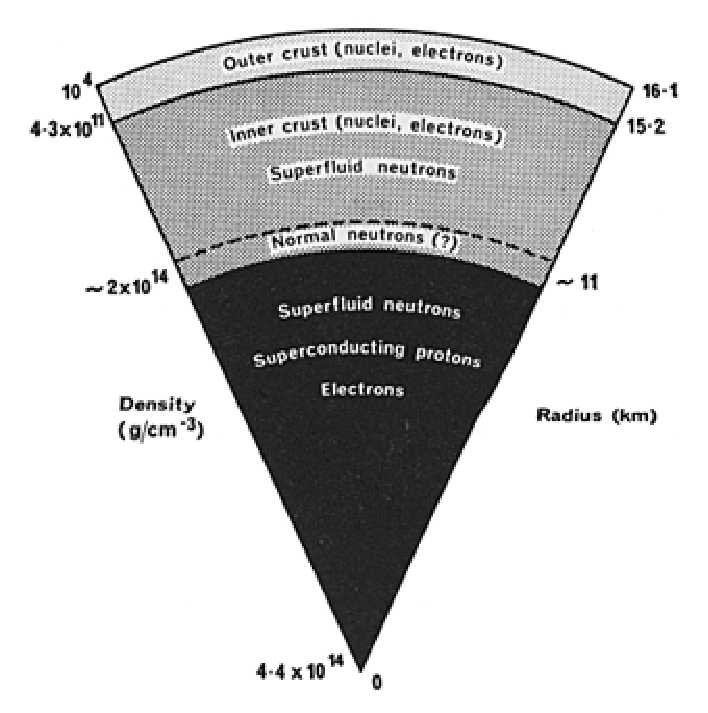
\includegraphics[height=111mm, width=148mm]{neutron_star_structure.eps}
	\caption{Hypothetical internal structure of a neutron star (Citation: \url{http://heasarc.gsfc.nasa.gov/docs/objects/binaries/neutron_star_structure.html})} 
        %CITE Possibly original Frank Shu? Fred would probably know, being a student of Frank
	\label{neutron_star_structure}
	\end{center}
	\end{figure}


    \section{Laser Interferometer Gravitational-wave Observatories}
    \label{LIGO}
        
        LIGO observatories. The most fun part to write. Cite Nergis Mavalvala~\cite{MavalvalaThesis}, Stefan Ballmer~\cite{BallmerThesis}, Rana Adhikari~\cite{AdhikariThesis}, Nicolas de Mateo Smith-Lefevbre~\cite{SmithThesis} and, of course, Peter Saulson~\cite{Saulson}.

        \subsection{From Weber bars to interferometry}
        \label{bars_to_interferometry}

            History lesson: Weber bars progress to interferometers. Use Saulson, but Nic's thesis has links to some of the original sources~\cite{Saulson},~\cite{SmithThesis}.           

        \subsection{Observatories, investigations, and enhancements}
        \label{methods}

		Michelson was one of the first to use interferometers~\cite{michelson}. He is famous for having done so to try to measure the velocity of the Earth with respect to the luminerferous ether and finding it to be unmeasurable.

A gravitational wave interferometer, at its core, is also a Michelson interferometer. 
The power $P$ at the output `dark' port, is by design equal to zero except when the measureable (e.g., ether, a gravitational wave, or other disturbance) causes a fringe shift $\Delta \phi$ related to the agnular frequency $\omega$ of the light and the time-of-flight down the $x$ and $y$ arms, $T_x$ and $T_y$. 
Physically, it is proportional to the electric field: 

\begin{eqnarray}
P \propto E_0^2 \left| 1 + e^{i \Delta \phi}\right|^2 = 2 E_0^2 (1 + \cos \Delta \phi), \\
\Delta \phi = \omega (T_y - T_x).
\end{eqnarray}

In Enhanced and Advanced LIGO, $\Delta \phi = 2\pi L_s /\lambda + \phi_0 + \phi_{\textup{DARM}} $, where in decreasing order of size, $L_s$ is known as the Schnupp asymmetry (a constant difference in arm length), $\phi_0$ is a constant offset from a fringe to enable non-radio-frequency-modulated DC readout, and $\phi_{\textup{DARM}}$ is the putative time-varying signal of `DARM', the differential arm motion that might encode a gravitational wave signal. 

Power $P$ can be directly improved by increasing effective laser power (e.g., a brighter laser or use of `power recycling'), and $\delta \phi$ can be increased by making $T_{x,y}$ storage times longer (e.g., with Fabry-Perot cavities).

Gravitational wave signals enter the interferometer, in a technical sense, by changing the spacetime curvature in the arms. It is not necessary to discuss mirror motion or Doppler shifting, although these are also valid points of view. 

In the simplest, linearized picture, the spacetime curvature leads to a gravitational wave with amplitude $h$; when the wave is aligned with x-axis and y-axis arms of length $L$ (see~\cite{Jaranowski1998} for the antenna pattern correction when it is misaligned), it changes the time-of-flight in the arms:

\begin{eqnarray}
T_x = \int_0^{\frac{2L_x}{c}} \sqrt{|g_{xx}|} dt \propto \int_0^{\frac{2L_x}{c}} \left(1 - \frac{h_+}{2} \right) dt, \\
T_y = \int_0^{\frac{2L_y}{c}} \sqrt{|g_{yy}|} dt \propto \int_0^{\frac{2L_y}{c}} \left(1 + \frac{h_+}{2} \right) dt.
\end{eqnarray}

\noindent The mismatch in the integrals leads to a detectable time-varying signal,

\begin{equation}
\phi_{\textup{DARM}} = \omega \int_0^{\frac{2L}{c}} \frac{h_+ (t, x(t)) + h_+ (t, y(t))}{2} dt.
\end{equation}  



            Why GW interferometers work. Null measurements, a zeroed operating point. The specifics are best handled by Saulson~\cite{Saulson}. The idea of a Pound-Drever-Hall lock is most elegantly explained by Black~\cite{PDHNotes}. Rai Weiss may have some neat details, possibly historical, albeit that it is in a presentation~\cite{LIGOWorks}. The details of Fabry-Perot cavities in LIGO are handled by Rakhmanov, Savage et al~\cite{ResonanceFP},~\cite{ResponsesFP}. The motivation for the evolution to Enhanced LIGO and its DC readout methods is covered well in the corresponding CQG article~\cite{Fricke2009} and specific details of its construction and operation are in Tobin Fricke's thesis~\cite{FrickeThesis}.

            \subsubsection{Interferometer theory}
            \label{interferometer_theory}
        
                GW interferometry theory: differential arm motion, key noise sources. Again, the main source is Saulson~\cite{Saulson}, although we also need another source in the Advanced Detector Era.

                Here we discuss the key noises sources: seismic noise, thermal noise, and quantum (radiation pressure, shot noise).

            \subsubsection{Observatory operation}
            \label{observatory_operation}

                Operating LIGO: controls, Detector Characterization. One of the first sources from initial LIGO to read up on is a paper by Fritscel, Bork, Mavalvala et al~\cite{ReadoutGWA}. Initially this system made a detection based on heterodyne readout using gravitational wave sidebands, which, among other troubles, could be unequal in the recycling cavity~\cite{MeadorsHanford2005}.

	\begin{figure}
	\begin{center}
	\includegraphics[height=111mm, width=148mm]{Screen_shot_2010-07-21_at_042516.eps}
	\caption{Screenshot of MEDM control panel}
	\label{ScreenshotMEDM}
	\end{center}
	\end{figure}


                \paragraph{Detector characterization}
                \label{detchar}
            
                    DetChar methods: omega scans, line hunting and glitches

                \paragraph{Feedforward filtering}
                \label{feedforward_filters}

                    Example of feedforward: 60 Hz magnetometer. The only source that mentions this is, I think, Nic's thesis~\cite{SmithThesis}. Yet the most pertinent example is one that has long been applied to LIGO: MICH and PRC feedforward. The specific needed are mention in the thesis of Adhikari~\cite{AdhikariThesis} and Ballmer~\cite{BallmerThesis}, but immediately before Keita Kawabe and I began our project, these parameters had been tuned by Jeff Kissel~\cite{KissellPRCMICH}

	\begin{figure}
	\begin{center}
	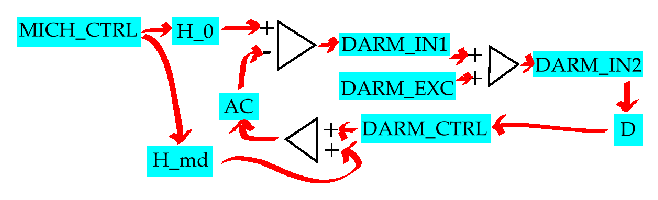
\includegraphics[height=111mm, width=148mm]{servo_loop.eps}
	\caption{Real-time servo loop diagram}
	\label{servo_loop_realtime}
	\end{center}
	\end{figure}

	\begin{figure}
	\begin{center}
	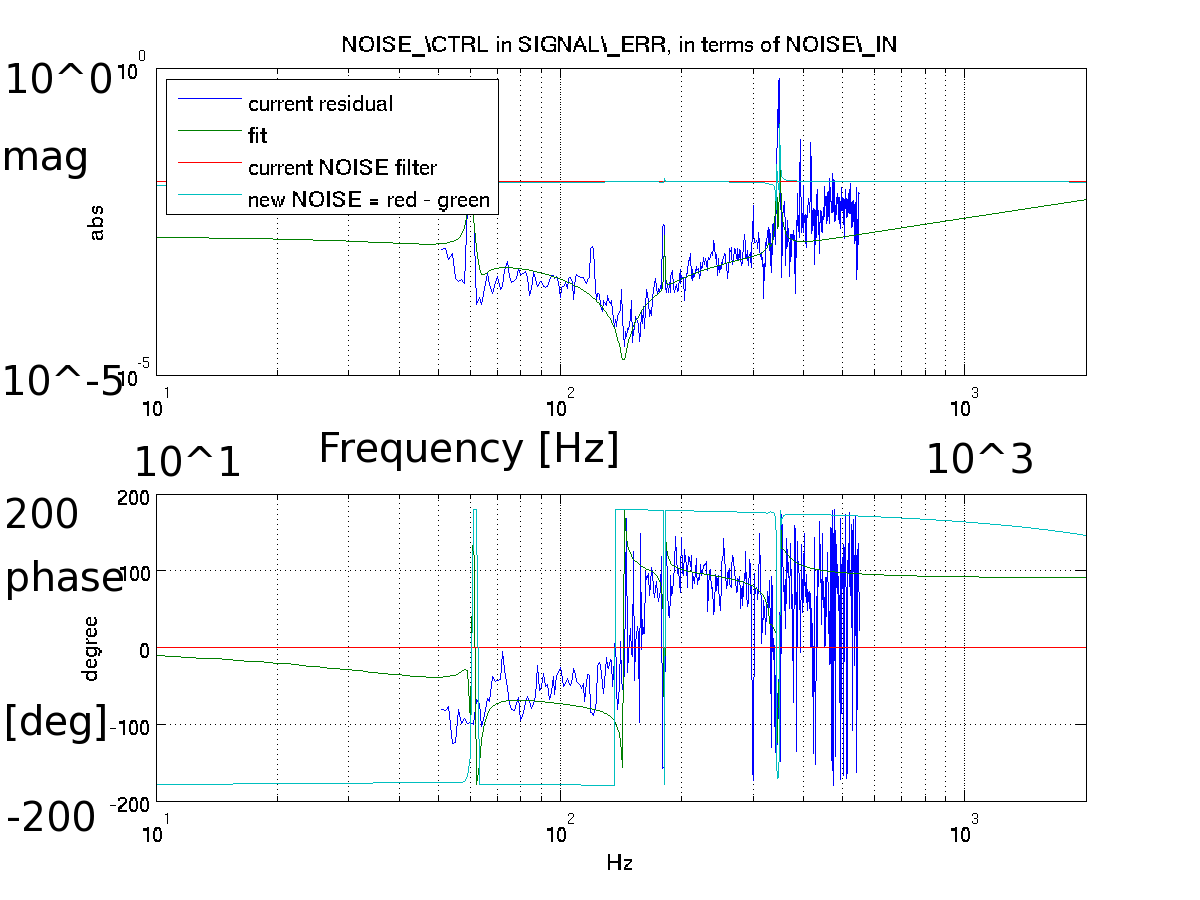
\includegraphics[height=111mm, width=148mm]{newNOISEfilter.eps}
	\caption{Real-time work on a LIGO noise filter}
	\label{newNOISEfilter}
	\end{center}
	\end{figure}

	\begin{figure}
	\begin{center}
	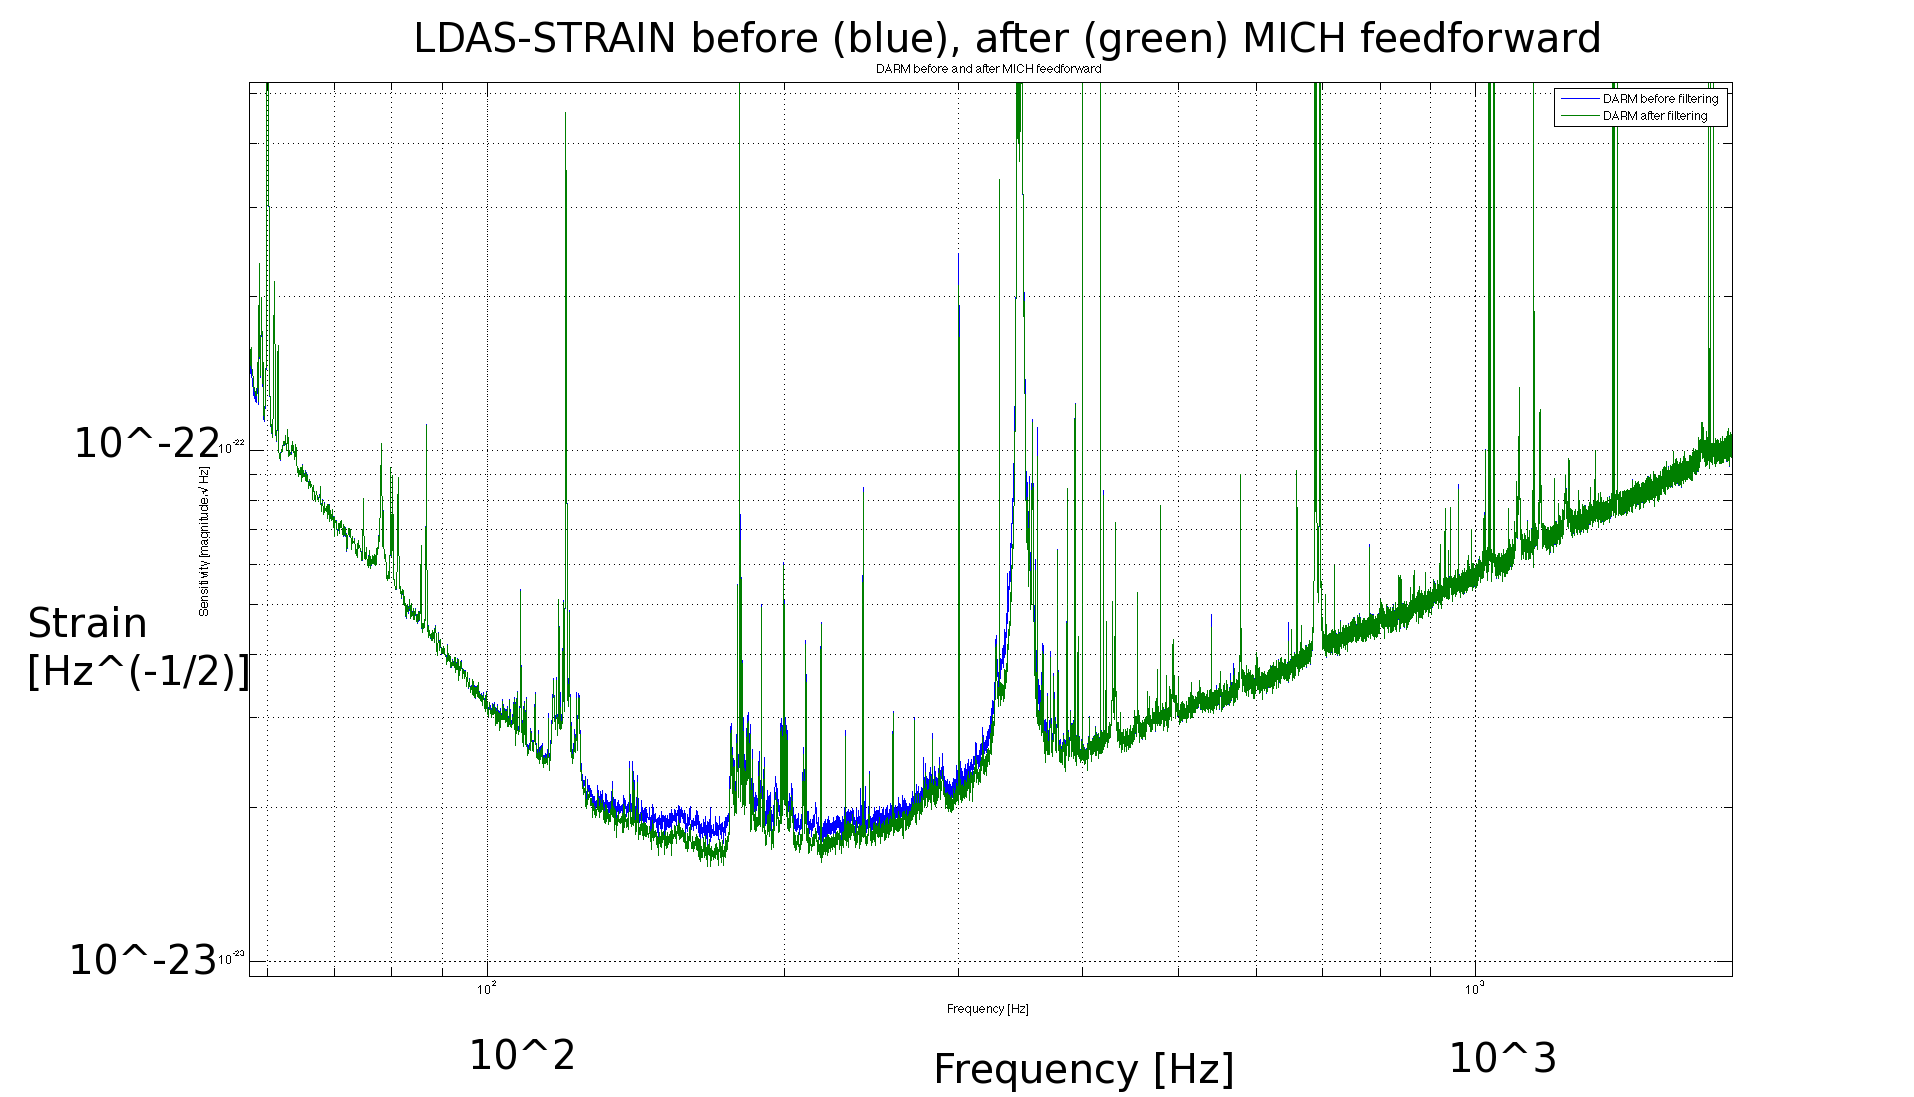
\includegraphics[height=111mm, width=148mm]{2011-03-08_filter-01.eps}
	\caption{Early work on post-facto noise filtering}
	\label{filter_early}
	\end{center}
	\end{figure}

                \paragraph{Phase camera}
                \label{phase_camera}

                    Future devices: overview of phase camera with Vladimir. Vladimir's thesis definitely talks about it~\cite{DergachevThesis}. We can discuss the fundamentals behind the need for angular stabilization and control from Nergis Mavalvala's thesis~\cite{MavalvalaThesis}, but we can refresh it with a modern reference from Kate Dooley's thesis~\cite{DooleyThesis}.


        \subsection{Advanced observatories and beyond}
        \label{advanced}
  
            Advanced LIGO and beyond -- squeezing and prospects?

        \subsection{Worldwide network}
        \label{worldwide}
 
            Allies: LIGO India, KAGRA, Advanced VIRGO, Einstein Telescope, LISA

    \section{Summary}
    \label{intro_summary}
 
        %Summary: strong motivation and instruments, need to find evidence of GW.    

Initial LIGO, during the science runs S6, would have been able to see the coalescence of two neutrons stars at about twenty Megaparsecs, out in the Virgo cluster of galaxies, from sixty-five million years ago, when dinosaurs still walked the Earth. 
In the first week of Advanced LIGO lock at Livingston, following Memorial Day 2014, Advanced LIGO had a temporal range extending only as far back as when early humans began their diaspora from Africa -- a terrestrial parallel to the expansion of the cosmos.
When completed, the Hanford and Livingston second-generation interferometers should see back ten times beyond what S6 could, six hundred and fiften million years, to before the Cambrian explosion of life.
Perhaps in the third or fourth generation of interferometers, our view of the gravitational sky may stretch back the age of the observable universe.
Even then, we will not have seen all that can be seen.
With the two long-range forces of the universe, electromagnetism and gravitational, giving two complimentary views of spacetime, we still must build great machines to explore the sights they show, we must understand what we are seeing, and we must propogate that understanding. 

This thesis is a prelude to those efforts, from the building of the quantum optical squeezer, and the feedforward regression and continuous waves binary search, to our public interferometer exhibitions.   
Feedforward regression provides a microcosm of the complexities of gravitational wave interferometry, so there we will begin.


            
%        --------------------
%
%	Here is a sample chapter file. The chapters of the thesis
%	should be saved to seperate files such as
%	\textit{chapter1.tex}. In the file \textit{thesis.tex} the
%	\textit{input} command then includes these chapters into the
%	thesis. Note that none of the chapter files need any headers.
%	This header for each of these files is contained in
%	\textit{thesis.tex}. The file \textit{thesis.tex} also
%	includes the numbers system for the sections, figures,
%	theorems lemmas etc...

%\section{Sample Section}
%\label{sample_section}
%
%	This is what a sample section looks like. Let's conclude this
%	section with a sample theorem statement and proof.
%
%	\begin{theorem}
%	\label{sample_theorem}
%	The are an infinite number of prime numbers
%	\end{theorem}
%
%	\emph{Proof:} On the contrary assume there are a finite number
%	of primes $P_1, P_2, ... P_n$. Consider $\mathcal{P} = P_1 P_2
%	\cdots P_n+1$. $\mathcal{P}$ is not divisible by any of the
%	primes in our finite set. (Contradiction) $\square$
  

